\documentclass[tikz]{standalone}
\tikzset{near start abs/.style={xshift=1cm}}

\usetikzlibrary{positioning}
\begin{document}
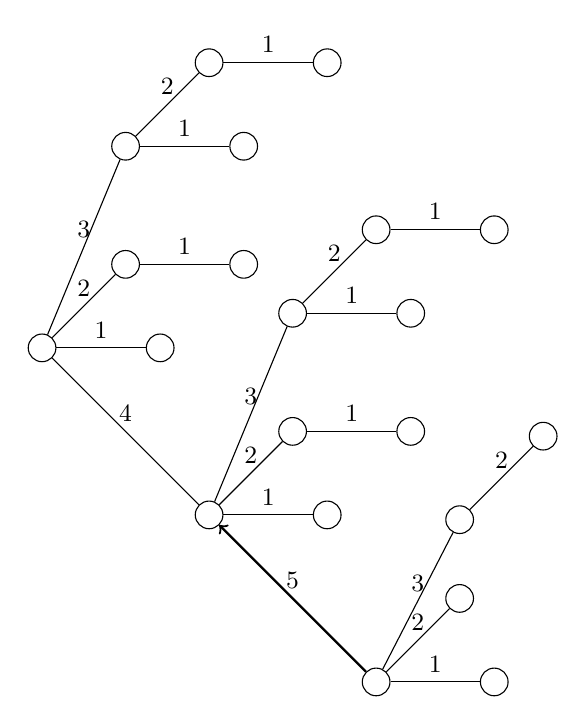
\begin{tikzpicture}[node distance=1.5cm]
    % place nodes
    \node[circle,draw=black, fill=white, inner sep=0pt,minimum size=10pt] (r) {};
    \node[circle,draw=black, fill=white, inner sep=0pt,right of=r, minimum size=10pt] (r1a)  {};
    \node[circle,draw=black, fill=white, inner sep=0pt,above right of=r, minimum size=10pt] (r2a)  {};
    \node[circle,draw=black, fill=white, inner sep=0pt,right of=r2a, minimum size=10pt] (r2b)  {};
    \node[circle,draw=black, fill=white, inner sep=0pt,above of=r2a, minimum size=10pt] (r3a)  {};
    \node[circle,draw=black, fill=white, inner sep=0pt,right of=r3a, minimum size=10pt] (r3b)  {};
    \node[circle,draw=black, fill=white, inner sep=0pt,above right of=r3a, minimum size=10pt] (r4a)  {};
    \node[circle,draw=black, fill=white, inner sep=0pt,right of=r4a, minimum size=10pt] (r4b)  {};
    % Extension from 7 nodes
    % Blank node
    \node[inner sep=0pt,below right of=r, minimum size=10pt] (t)  {};
    
    \node[circle,draw=black, fill=white, inner sep=0pt,below right of=t, minimum size=10pt] (t1)  {};
    \node[circle,draw=black, fill=white, inner sep=0pt,right of=t1, minimum size=10pt] (t1a)  {};
    \node[circle,draw=black, fill=white, inner sep=0pt,above right of=t1, minimum size=10pt] (t2a)  {};
    \node[circle,draw=black, fill=white, inner sep=0pt,right of=t2a, minimum size=10pt] (t2b)  {};
    \node[circle,draw=black, fill=white, inner sep=0pt,above of=t2a, minimum size=10pt] (t3a)  {};
    \node[circle,draw=black, fill=white, inner sep=0pt,right of=t3a, minimum size=10pt] (t3b)  {};
    \node[circle,draw=black, fill=white, inner sep=0pt,above right of=t3a, minimum size=10pt] (t4a)  {};
    \node[circle,draw=black, fill=white, inner sep=0pt,right of=t4a, minimum size=10pt] (t4b)  {};
    
    % Third group
    \node[inner sep=0pt,below right of=t1, minimum size=10pt] (v)  {};
    
    \node[circle,draw=black, fill=white, inner sep=0pt,below right of=v, minimum size=10pt] (v1)  {};
    \node[circle,draw=black, fill=white, inner sep=0pt,right of=v1, minimum size=10pt] (v1a)  {};
    \node[circle,draw=black, fill=white, inner sep=0pt,above right of=v1, minimum size=10pt] (v2a)  {};
    \node[circle,draw=black, fill=white, inner sep=0pt,above right of=v1,yshift=1cm, minimum size=10pt] (v3a)  {};
    \node[circle,draw=black, fill=white, inner sep=0pt,above right of=v3a, minimum size=10pt] (v4a)  {};
    \draw (r) -- node[above] {\small{1}} ++(r1a);
    \draw (r) -- node[above] {\small{2}} ++(r2a);
    \draw (r3a) -- node[above] {\small{3}} ++(r);
    \draw (r2a) -- node[above] {\small{1}} ++(r2b);
    \draw (r3a) -- node[above] {\small{1}} ++(r3b);
    \draw (r3a) -- node[above] {\small{2}} ++(r4a);
    \draw (r4a) -- node[above] {\small{1}} ++(r4b);
    
    % Second nodes
    \draw (t1) -- node[above] {\small{1}} ++(t1a);
    \draw (t1) -- node[above] {\small{2}} ++(t2a);
    \draw (t3a) -- node[above] {\small{3}} ++(t1);
    \draw (t2a) -- node[above] {\small{1}} ++(t2b);
    \draw (t3a) -- node[above] {\small{1}} ++(t3b);
    \draw (t3a) -- node[above] {\small{2}} ++(t4a);
    \draw (t4a) -- node[above] {\small{1}} ++(t4b);
    
    % Third node
    \draw (v1) -- node[above] {\small{1}} ++(v1a);
    \draw (v1) -- node[above] {\small{2}} ++(v2a);
    \draw (v3a) -- node[above] {\small{3}} ++(v1);
    \draw (v4a) -- node[above] {\small{2}} ++(v3a);
    \draw (r) -- node[above] {\small{4}} ++(t1);
    \draw[->, thick] (v1) -- node[above] {\small{5}} ++(t1);
    % \draw (t1) -- node[above] {\small{3}} ++(t2a);
    % \draw (t1) -- node[above] {\small{2}} ++(t2b);
\end{tikzpicture}
\end{document}